\section{Экспериментальное исследование}

Для экспериментальной проверки разработанного программного средства были проведены две серии экспериментов. Первая серия проведена для сравнения разработанного программного средства с наивным байесовским классификатором, используемым во многоих открытых системах фильтрации спама.

Вторая серия экспериментов проведена для проверки работы системы в многопрофильном режиме.

\subsection{Сравнение с наивным байесовским классификатором}

\subsubsection {Набор данных}

Тестирование производилось на двух публичных наборах email-сообщений.

\begin{enumerate}
	\item SpamAssassin public corpus \cite{SAPC}
	\item CEAS 2008 Live Spam Challenge Laboratory Corpus \cite{CEAS}
\end{enumerate}

\subsubsection{Методика тестирования}

Тестирование производилось с использованием метода скользящего контроля: выборка разбивалась на пять частей, на четырех из которых проводилось обучение, а на пятой - контроль. Выборка \cite{CEAS} ввиду своей большой величины была разделена на несколько частей, на каждой из которых тестирование было произведено отдельно. 

Результат тестирования представлен в виде графика соответствия величин вероятности ложно-положительного срабатывания и вероятности верного обнаружения спама. Точка на графике обозначает что при определенной границе решающего правила система будет работать именно в таком режиме: фильтровать спам с вероятностью показанной на оси ординат и классифицировать легитимные письма как спам с вероятностью показанной на оси абцисс. Чем выше проходит график, тем более качественно работает система фильтрации.

\subsubsection{Результаты тестирования}
На графиках \ref{SAPCBAYESSVM} и \ref{CEASBAYESSVM} представлены результаты тестирования на наборах \cite{SAPC} и \cite{CEAS}. Видно, что разработанное средство всегда работает лучше чем наивный байесовский классфикатор.

\begin{figure}[h]
\begin{center}
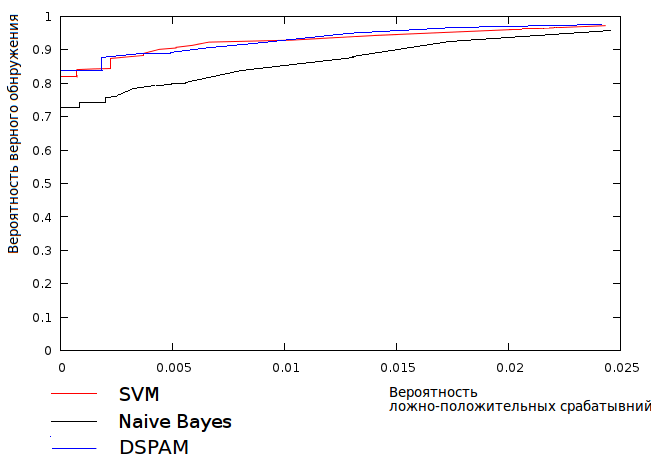
\includegraphics[width=15cm]{img/graphic}
\end{center}
\caption{Сравнение качества тестирования реализованного алгоритма и наивного байесовского классификатора на наборе \cite{SAPC}}
\label{SAPCBAYESSVM}
\end{figure}

\begin{figure}[h]
\begin{center}
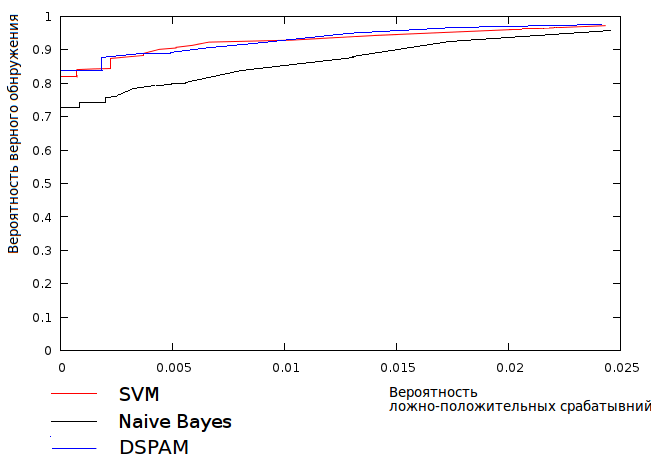
\includegraphics[width=15cm]{img/graphic}
\end{center}
\caption{Сравнение качества тестирования реализованного алгоритма и наивного байесовского классификатора на наборе \cite{SAPC}}
\label{CEASBAYESSVM}
\end{figure}

\subsection{Тестирование работы в многопрофильном режиме}

\subsubsection{Набор данных}
Тестирование производилось на наборе данных SpamAssassin Public Corpus

\subsubsection{Методика тестирования}

\subsubsection{Результаты}

